\documentclass{article}
\usepackage[demo]{graphicx}
\usepackage[format=hang,singlelinecheck=0,font={sf,small},labelfont=bf]{subfig}
\usepackage{caption}
\usepackage[noabbrev]{cleveref}

\graphicspath{{figures/}}

\captionsetup[subfigure]{subrefformat=simple,labelformat=simple,listofformat=subsimple}
\renewcommand\thesubfigure{(\alph{subfigure})}

\begin{document}

\begin{figure}
\centering
%\captionsetup{justification=raggedright}
\subfloat[text]{\label{fig:1a}\includegraphics{file1.eps}}\qquad
\subfloat[text]{\label{fig:1b}\includegraphics{file2.eps}}\\
\subfloat[text]{\label{fig:1c}\includegraphics{file3.eps}}\qquad
\subfloat[text]{\label{fig:1d}\includegraphics{file4.eps}}
\caption{\protect\subref{fig:1a} to \protect\subref{fig:1b} are plotted against height, and \protect\subref{fig:1c} to \protect\subref{fig:1d} against pressure}
\label{fig:1}
\end{figure}


Now I refer to the figure \subref*{fig:1d}. And use cref: \cref{fig:1d} and also \subref{fig:1d}

\end{document}

\begin{figure}[ht]
	\centering
	\subfigure[Main alignment mark at 5x magnification]{
		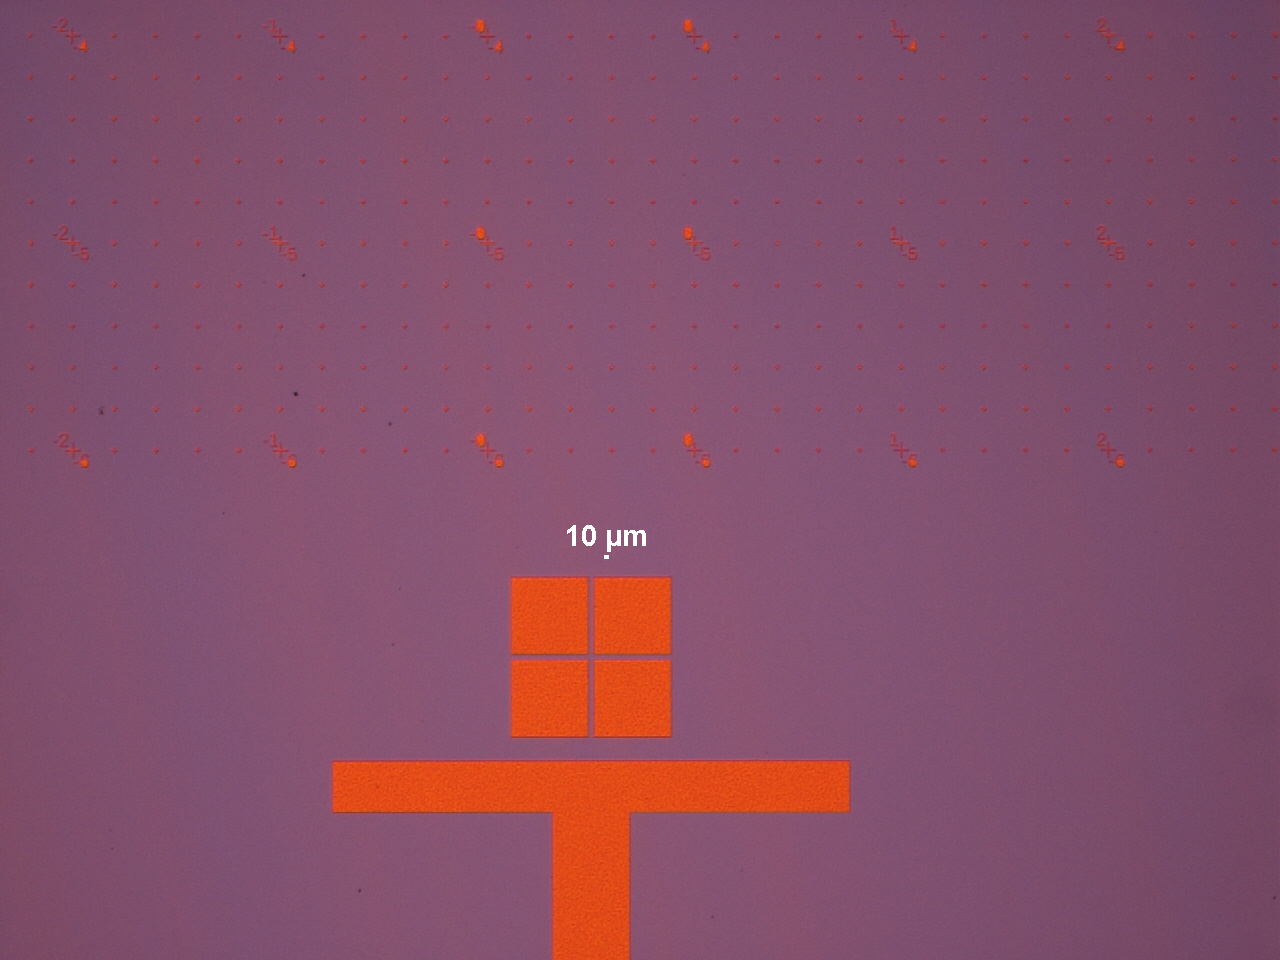
\includegraphics[height=4cm,width=5cm]{figs/experimental/main_alignment_5x}
		\label{fig:main_alignment_5x}
		}
	\qquad
	\subfigure[Main alignment mark at 10x magnification]{
		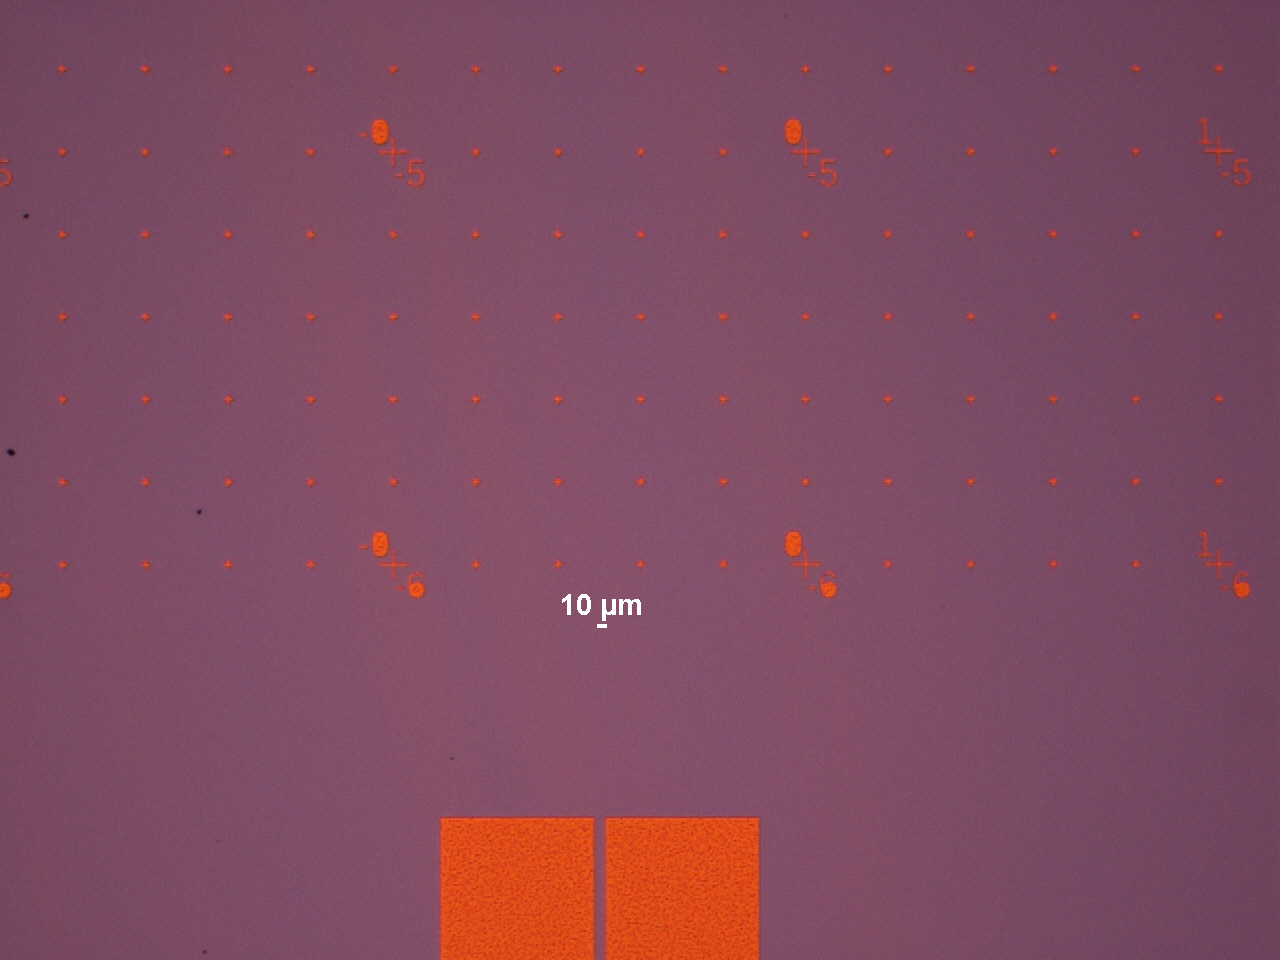
\includegraphics[height=4cm,width=5cm]{figs/experimental/main_alignment_10x}
		\label{fig:main_alignment_10x}
		}

	\subfigure[Coordinate mark $\left(0,-5\right)$ at 50x magnification]{
		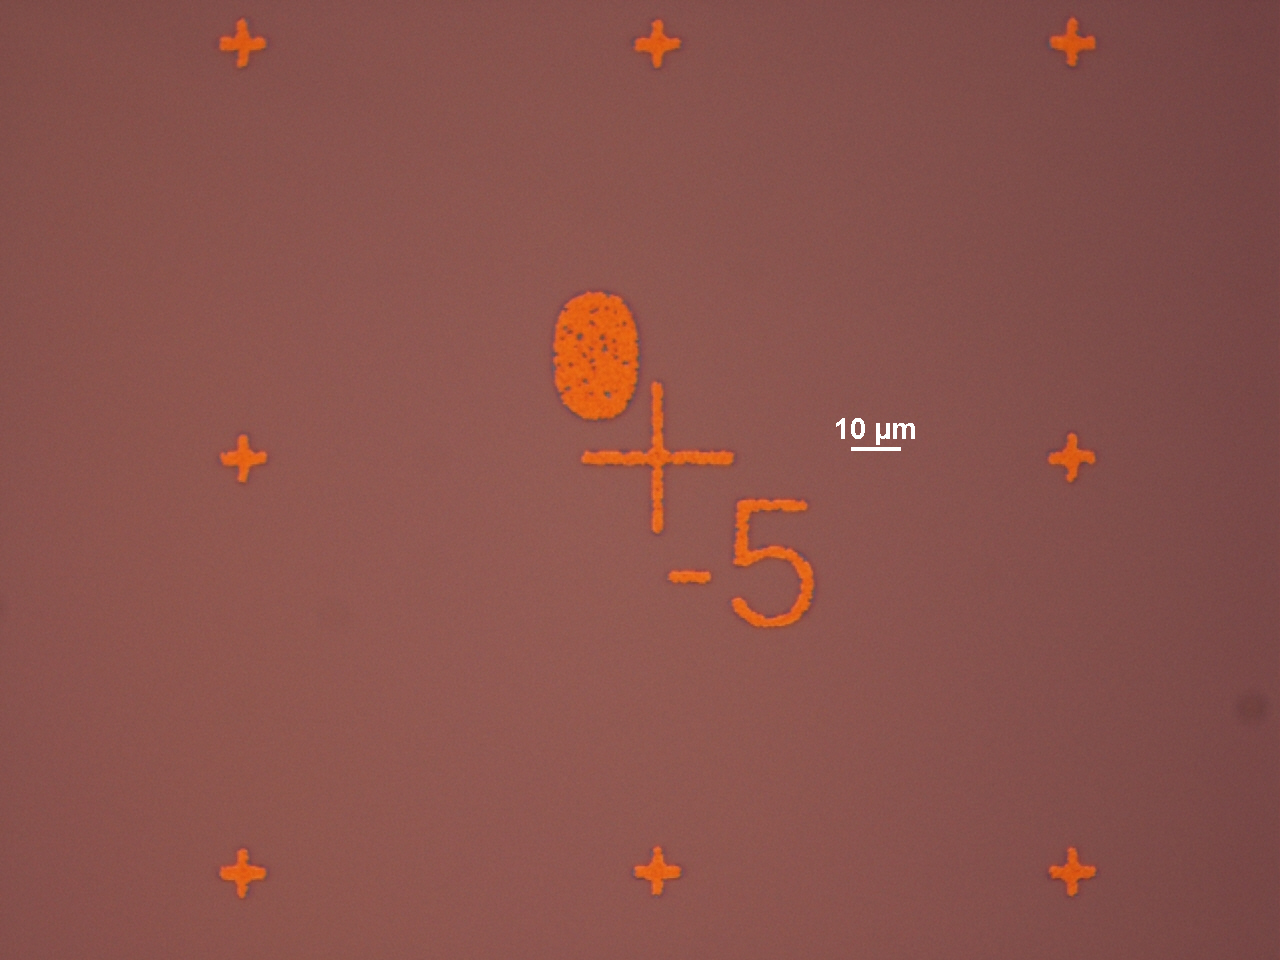
\includegraphics[height=4cm,width=5cm]{figs/experimental/main_alignment_50x}
		\label{fig:main_alignment_50x}
		}
	\qquad
	\subfigure[Coordinate mark $\left(0,-5\right)$ at 100x magnification]{
		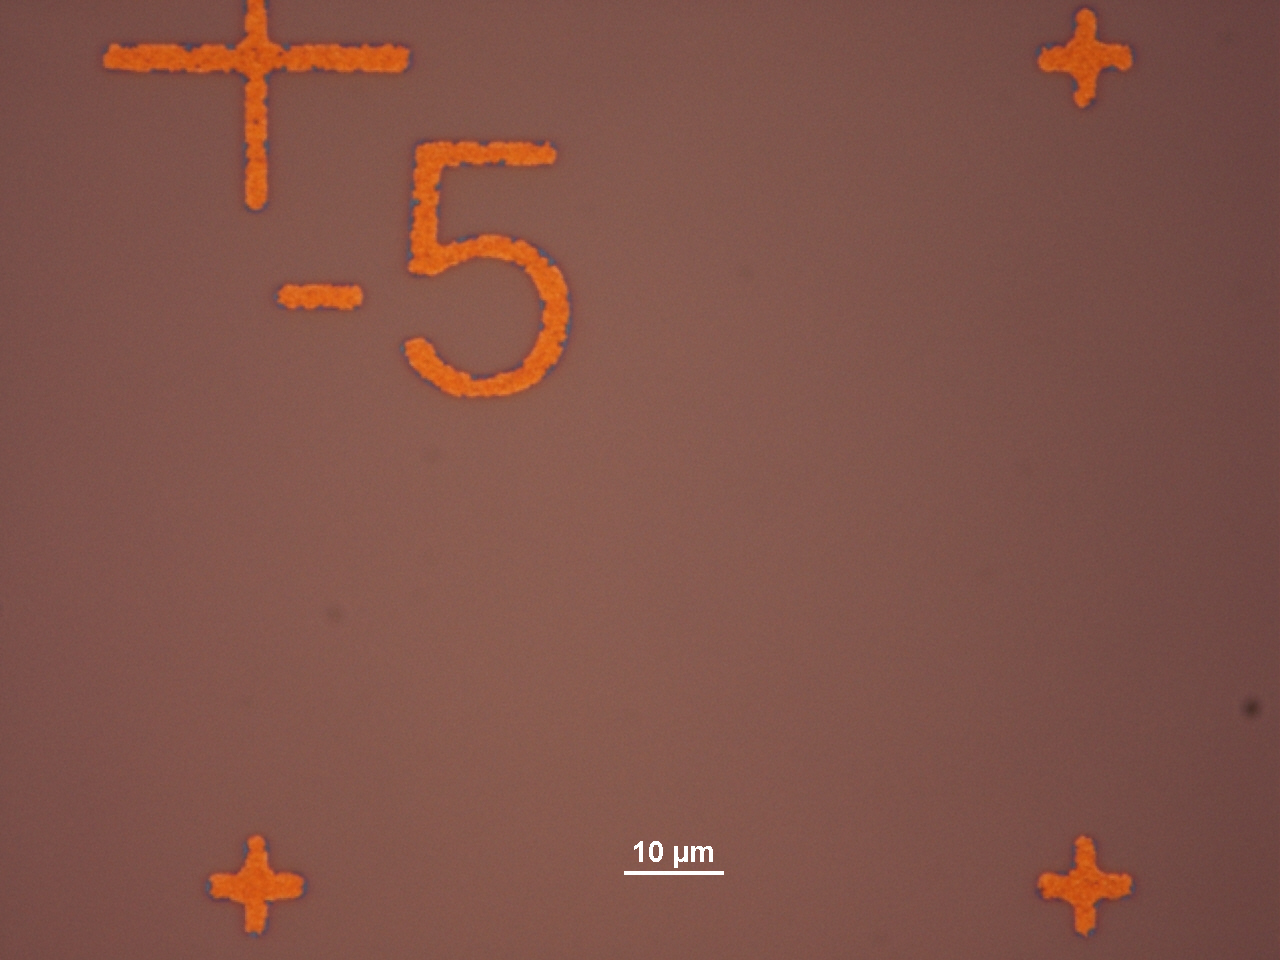
\includegraphics[height=4cm,width=5cm]{figs/experimental/main_alignment_100x}
		\label{fig:main_alignment_100x}
	}
	\caption[Alignment marks at varying magnifications]{Main alignment mark and a coordinate point on a substrate at various magnifications}
	\label{fig:main_alignment}
\end{figure}
